\documentclass[a4paper,12pt,exos,firamath]{nsi}
		
\setminted{fontsize=\small}
\begin{document}
{\large\bfseries \scshape Nom Prénom : \makebox[6cm]{\dotfill}\hfill Heure de passage : \makebox[3cm]{\dotfill}\hfill\\
\vspace{2em}
\hrule
\vspace{2mm}
\begin{center}\titlefont\Huge\color{UGLiBlue} BTS SIO\\
	Sous-épreuve E22 \\ 
    Algorithmique appliquée\\
	Contrôle en Cours de Formation\end{center}
\vspace{2mm}
\hrule}
\vspace{2em}

\begin{encadrecolore}{Déroulement de l'épreuve }{UGLiGreen}
	Cette épreuve de Contrôle en cours de Formation (CCF) se déroule en trois étapes :
\begin{itemize}
	\item \textbf{\'Etape 1 : \'Ecrit (30 minutes)}\par
	Vous devez traiter la partie A du sujet. Pour cette partie, l'ordinateur est interdit mais la calculatrice est autorisée.\\
    
    \textbf{Vous inscrirez vos réponses dans le document réponse à la fin du sujet.}\\
    
    Les algorithmes à écrire peuvent être rédigés en \textbf{langage naturel} ou en \textsc{Python}	mais ni en \textsc{C\#} ni en \textsc{VB.Net}.\\
    
    \textbf{À la fin de l'étape 1, votre document réponse doit être remis à la personne surveillant l'épreuve.} Vous garderez le sujet.
    \item \textbf{\'Etape 2 : sur machine (30 minutes)}\par
	Vous devez traiter la partie B du sujet à l'aide d'un ordinateur. Le langage utilisé est celui travaillé dans l'année, à savoir \textsc{Python}.
	Vous sauvegarderez votre travail sur la clé USB fournie.\par 
	La durée totale pour effectuer les deux premières étapes est exactement d'une heure. \par
	\item \textbf{\'Etape 3 : oral (20 minutes au maximum)}\\
	Cette partie se déroule en deux temps. Tout d'abord, vous disposez de 10 minutes pour présenter votre travail de l'étape 2 puis, au cours des 10 minutes suivantes, un entretien permet de préciser votre démarche.
\end{itemize}	

\textbf{À la fin de l'épreuve le sujet devra être rendu à l'examinateur.}
\end{encadrecolore}
\newpage
\titre{ Compression RLE}
\classe{CCF Algo SIO}
\maketitle


Une image en noir et blanc peut être représentée par une liste d'entiers valant 0 (pour le noir) et 1 (pour le blanc).\\
Par exemple l'image suivante, de dimensions $3\times 4$ 
\begin{center}
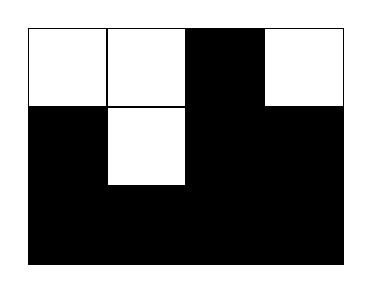
\begin{tikzpicture}
\draw[fill=black!0] (0,2) rectangle (1,3);
\draw[fill=black!0] (1,2) rectangle (2,3);
\draw[fill=black] (2,2) rectangle (3,3);
\draw[fill=black!0] (3,2) rectangle (4,3);
\draw[fill=black] (0,1) rectangle (1,2);
\draw[fill=black!0] (1,1) rectangle (2,2);
\draw[fill=black] (2,1) rectangle (3,2);
\draw[fill=black] (3,1) rectangle (4,2);
\draw[fill=black] (0,0) rectangle (1,1);
\draw[fill=black] (1,0) rectangle (2,1);
\draw[fill=black] (2,0) rectangle (3,1);
\draw[fill=black] (3,0) rectangle (4,1);
\end{tikzpicture}
\end{center}

est représentée par la liste obtenue en parcourant les pixels de gauche à droite et du haut vers le bas :

\mint{python}{[1, 1, 0, 1, 0, 1, 0, 0, 0, 0, 0, 0]}

C'est une liste de longueur 12 car l'image comporte $3\times 4 = 12$ pixels.\\


L'objectif de ce sujet est de compresser l'image, c'est-à-dire d'obtenir une liste plus courte qui nous permet de retrouver l'image. Pour simplifier l'image sera toujours de dimension $3\times 4$.

On utilise la méthode suivante :
\begin{itemize}
	\item on commence au début de la liste et on compte les zéros ;
    \item puis on compte le nombre de uns ;
    \item et ainsi de suite jusqu'à la fin de la liste.
\end{itemize}
Par exemple avec la liste précédente :
\begin{itemize}
	\item on commence par compter les zéros : il y en a... zéro !
    \item puis 2 uns ;
    \item puis 1 zéro ;
    \item puis 1 un ;
    \item et ainsi de suite.
\end{itemize}
On obtient la liste compressée suivante :
\mint{python}{[0, 2, 1, 1, 1, 1, 6]}

Elle est bien plus courte que la liste de départ car sa longueur est 7.

\begin{definition}
Le taux de compression $T$ (en pourcentage) d'une liste est défini par
$$T = 100\times\left(1 - \dfrac{\text{longueur de la liste compressée}}{\text{longueur de la liste}}\right)$$
\end{definition}

Par exemple le taux de compression dans la situation précédente est

$$100\times\left( 1-\dfrac{7}{12}\right)\simeq 41,6\%$$

\section*{\'Etape 1}

\begin{encadrecolore}{Question 1}{UGLiOrange}
Pour l'image suivante :
\begin{center}
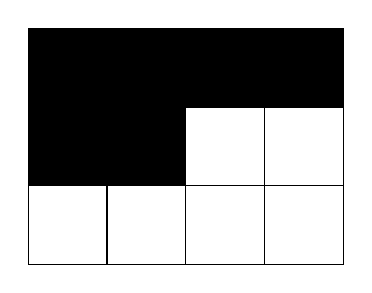
\begin{tikzpicture}
\draw[fill=black] (0,2) rectangle (1,3);
\draw[fill=black] (1,2) rectangle (2,3);
\draw[fill=black] (2,2) rectangle (3,3);
\draw[fill=black] (3,2) rectangle (4,3);
\draw[fill=black] (0,1) rectangle (1,2);
\draw[fill=black] (1,1) rectangle (2,2);
\draw (2,1) rectangle (3,2);
\draw (3,1) rectangle (4,2);
\draw (0,0) rectangle (1,1);
\draw (1,0) rectangle (2,1);
\draw (2,0) rectangle (3,1);
\draw (3,0) rectangle (4,1);
\end{tikzpicture}
\end{center}
\begin{enumalph}
	\item Donner la liste associée.
    \item Donner la liste compressée.
    \item Quel est le taux de compression ?
\end{enumalph}
\end{encadrecolore}

\begin{encadrecolore}{Question 2}{UGLiOrange}
Refaire la même chose avec l'image suivante :
\begin{center}
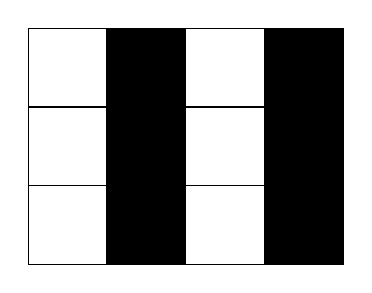
\begin{tikzpicture}
\draw (0,2) rectangle (1,3);
\draw[fill=black] (1,2) rectangle (2,3);
\draw (2,2) rectangle (3,3);
\draw[fill=black] (3,2) rectangle (4,3);
\draw (0,1) rectangle (1,2);
\draw[fill=black] (1,1) rectangle (2,2);
\draw (2,1) rectangle (3,2);
\draw[fill=black] (3,1) rectangle (4,2);
\draw (0,0) rectangle (1,1);
\draw[fill=black] (1,0) rectangle (2,1);
\draw (2,0) rectangle (3,1);
\draw[fill=black] (3,0) rectangle (4,1);
\end{tikzpicture}
\end{center}
\end{encadrecolore}

L'algorithme de compression est en partie donné :
\newpage


\begin{minted}[linenos]{pseudocode}
fonction compresse(ligne)

    variables
        résultat : liste
        valeur, compteur, i : entiers
        
    résultat ← liste vide
    valeur ← 0              # on part de la valeur 0
    compteur ← 0            # au départ il y en a zéro
    i ← 0                   # on commence au début de la ligne
    tant que i < longueur(ligne)
        si ligne[i] = ......
            compteur ← compteur + 1
        sinon
            valeur ← 1 - valeur
            ajouter compteur à la fin de résultat
            compteur ← 1
        .......
    ajouter compteur à la fin de résultat
    renvoyer résultat
\end{minted}

\begin{encadrecolore}{Question 3}{UGLiOrange}
\begin{enumalph}
	\item Si, juste avant d'exécuter la ligne 15, \texttt{valeur} vaut zéro, que devient \texttt{valeur} après l'exécution de la ligne 15 ?
    \item Même question si \texttt{valeur} vaut 1.
    \item Quel est le rôle de cette ligne ?
\end{enumalph}
\end{encadrecolore}


\begin{encadrecolore}{Question 4}{UGLiOrange}
Compléter l'algorithme.
\end{encadrecolore}


\begin{encadrecolore}{Question 5}{UGLiOrange}
Dessiner l'image qui produit la liste compressée
\mint{python}{[3,3,3,3]}
\end{encadrecolore}


\section*{\'Etape 2}

Le fichier \texttt{rle.py} contient l'implémentation en \textsc{Python} de la fonction \texttt{compresse} ainsi que 2 listes de test.


\begin{encadrecolore}{Question 7}{UGLiOrange}
Implémenter la fonction \texttt{taux\_de\_compression} qui
\begin{itemize}
	\item en entrée prend une liste composée de 0 et de 1 ;
    \item renvoie le taux de compression quand on compresse la liste.
\end{itemize}
\end{encadrecolore}


\begin{encadrecolore}{Question 8}{UGLiOrange}
Implémenter la fonction \texttt{decompresse} qui
\begin{itemize}
	\item en entrée prend une liste compressée ;
    \item renvoie la liste décompressée.
\end{itemize}
\end{encadrecolore}

\end{document}